\documentclass[a4paper,12pt]{scrartcl}
\usepackage{exercice_sheet}

%\trait
%\section*{}
%\exo{}
%\question{}
%\subquestion{}



\date{}

\newcommand{\classe}{prépa}
\newcommand{\typedevoir}{Évaluation} 
\newcommand{\duree}{}

\renewcommand{\hascorrection}{0}


% Title Page
\title{\typedevoir{} -- \classe{}\writecorrword{}} 

% \author{Durée : \duree{}}


\begin{document}

\maketitle

%\tableofcontents

Calculatrice autorisée. 

La difficulté du devoir n'est pas croissante: si vous bloquez sur un exercice ou une question, ne perdez pas trop de temps et allez à la suite.

\exo{Simplifications de racines carrées}
Simplifier les racines suivantes, c'est-à-dire les écrire avec un nombre le plus petit possible sous la racine voire, lorsque c'est possible, sans racine:

\question{$\sqrt{48}$}

\correction{$4\sqrt{3}$}

\lignes{3}

\question{$\sqrt{25}$}

\correction{$5$}

\lignes{3}

\question{$\sqrt{108}$}

\correction{$6\sqrt{3}$}

\lignes{3}

\exo{Puissances}
Simplifier les écritures suivantes:

\question{$10^4 \times 10^3$}

\correction{$10^{7}$}

\lignes{2}

\question{$10^2 \times 10^{-2}$}

\correction{$10^0=1$}

\lignes{2}

\question{$\dfrac{2^6}{2^3}$}

\correction{$2^3=8$}

\lignes{2}

\exo{Équations du premier degré à une inconnue}
Résoudre les équations suivantes:

\question{$4x-4 = 0$}

\correction{$\mathcal{S} = \left\{ 1 \right\}$}

\lignes{3}

\question{$3x+4 = 10$}

\correction{$\mathcal{S} = \left\{ 2 \right\}$}

\lignes{3}

\question{$8x+5 = 9$}

\correction{$\mathcal{S} = \left\{ \dfrac{1}{2} \right\}$}

\lignes{3}

\question{$\dfrac{1}{2} x + 2 = 7$}

\correction{$\mathcal{S} = \left\{ 10 \right\}$}

\lignes{3}

\exo{Fractions}
Simplifier les fractions suivantes:

\question{$\dfrac{4}{8}$}

\correction{$\dfrac{1}{2}$}

\lignes{3}

\question{$\dfrac{25}{15}$}

\correction{$\dfrac{5}{3}$}

\lignes{3}

\question{$\dfrac{10}{30}$}

\correction{$\dfrac{1}{4}$}

\lignes{3}

\question{$\dfrac{144}{12}$}

\correction{$12$}

\lignes{3}

\exo{Mise en équation}
Mettre en équation l'exercice suivant, puis résoudre:

Trouver cinq nombres entiers consécutifs dont la somme est 1515.

\correction{Appelons $n$ le premier des 5 nombres consécutifs.

    Les quatre suivants sont alors $n+1$, $n+2$, $n+3$ et $n+4$.

    On a donc l'équation:

    $$n+(n+1)+(n+2)+(n+3)+(n+4) = 1515 \Leftrightarrow 5n + 10 = 1515 \Leftrightarrow n = 301$$
}

\lignes{4}

\exo{Polynômes du second degré}
Résoudre les équations suivantes:

\question{$x^2 - x - 2 = 0$}

\correction{$\mathcal{S} = \left\{ -1;2 \right\}$}

\lignes{4}

\question{$x^2 - 5x + 6 = 0$}

\correction{$\mathcal{S} = \left\{2 ;3 \right\}$}

\lignes{4}

\question{$x^2 - 2x = 11 $}

\correction{$\mathcal{S} = \left\{ 1-2 \sqrt{3};1+2 \sqrt{3} \right\}$}

\lignes{4}


\exo{Géométrie (opticiens uniquement)}

\question{}
Quel théorème utilise-t-on pour calculer un côté d'un triangle rectangle lorsqu'on connaît les deux autres?

\correction{Le théorème de Pythagore}

\lignes{1}

\question{}
Soit le triangle ABC ci-dessous rectangle en $C$.

\begin{center}
    \begin{tikzpicture}[scale=1.5]
        \draw (0,0) -- (5,0);
        \draw (0,0) -- (1.8,2.4);
        \draw (5,0) -- (1.8,2.4);

        \draw (0,0)     node [below] {$A$};
        \draw (5,0)     node [below] {$B$};
        \draw (1.8,2.4) node [above] {$C$};
    \end{tikzpicture}
\end{center}

Sachant que $AC = 3$cm et $AB = 5$cm, calculer la longueur du côté $[BC]$.

\correction{D'après le théorème de Pythagore: $AB^2 = AC^2+BC^2$, d'où $BC^2 = AB^2 - AC^2$.

Donc $BC = \sqrt{AB^2 - AC^2} = \sqrt{25-9} = \sqrt{16} = 4$.

La longueur du côté $[BC]$ est donc de 4cm.}

\lignes{3}

\exo{Trigonométrie (opticiens uniquement)}

\question{}
Donner les valeurs suivantes (valeurs \emph{exactes}): 

\begin{itemize}
    \item $\sin 0$, 
        \correction{\item $\sin 0 = 0$}
    \item $\sin \frac{\pi}{2}$, 
        \correction{\item $\sin \frac{\pi}{2} = 1$}
    \item $\cos 0$, 
        \correction{\item $\cos 0 = 1$}
    \item $\cos \frac{\pi}{2}$
        \correction{\item $\cos \frac{\pi}{2} = 0$}
    \item $\sin \frac{\pi}{4}$, 
\end{itemize}

\lignes{3}

\question{}
Soit le triangle $ABC$ rectangle en $A$ ci-dessous:

\begin{center}
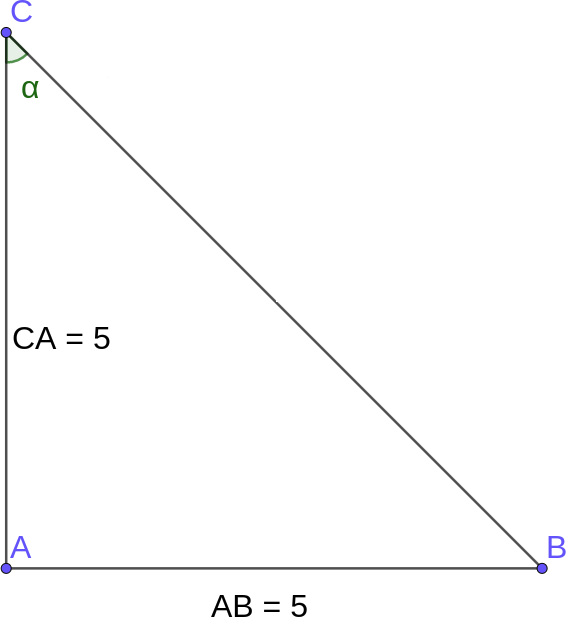
\includegraphics[width=0.4\linewidth]{pics/Triangle.png}
\end{center}

\subquestion{}
Exprimer $\tan \alpha$ en fonction de deux côtés du triangle, calculer la valeur de $\tan \alpha$ et en déduire $\alpha$. Valeur \emph{exacte} en radians ou en degrés acceptée.

\correction{$\tan \alpha = \dfrac{AB}{CA} = \dfrac{5}{5} = 1$, d'où $\alpha = \dfrac{\pi}{4} = \ang{45}$.} 

\lignes{2}

\subquestion{}
Calculer la longueur du côté $BC$, arrondie au dixième.

\correction{D'après le théorème de Pythagore, $BC^2 = AC^2+AB^2$ d'où $BC = \sqrt{AC^2+AB^2} = \sqrt{5^2+5^2} = \sqrt{50} = 5 \sqrt{2} \approx 7.1$.}

\lignes{2}

\end{document}

